\chapter{Introduction}
\label{introduction}
Music streaming services have an immense amount of power in the music industry. The biggest streaming services dictate the rules which artists have to play by. The top 5 streaming services and the top 3 labels dominate the market. Artists have a hard time to make a living because the streaming companies take large revenue cuts. The centralization of power on Internet platforms cause unfairness in multiple industries, of which the music industry is particularly affected. This thesis aims to distribute the power from centralized streaming platforms to listeners and artists.

The music streaming industry is completely digital\; from recording and publishing to listening and digital rights management. We investigate the feasibility of fully replacing this digital value chain by software. 

\todo[inline]{Insert clear Robot Economy definition, Insert contributions and goals of this thesis}
% Een problem begin zoals dit:
% The robot economy is already here.Instead, we are still suffering big stagnation; income polarisation is rapidly increasing, wages have been falling, and the rate of technological progress is slowing down. In addition, the latest wave of digital innovation has resulted in excessive returns to capital, with a massive amount of cash going to the balance sheets of big tech companies, while very little is invested in welfare, social infrastructures, education, health and clean energy. This situation is exacerbated by the apparent inability of governments to tax profits made by hi-tech and financial giants, as seen, for instance, in the very generous tax settlement between Google and the government. 
% https://www.opendemocracy.net/en/can-europe-make-it/robot-economy-full-automation-work-future/

\section{Monopolization on the Internet}
The Internet is moving from a network of people to a sparse selection of platforms over which nearly all commerce is regulated. A few Big Tech corporations are gaining increasing power in the the surface on which market exchange takes place. The consumer choice is diminishing due to the power of oligarchs and monopolies. As explained by \citep{stiglitz2019market}, there is a fundamental problem: the growing ``concentration of market power, which allows dominant firms to exploit their customers and squeeze their employees, whose own bargaining power and legal protections are being weakened'', while ``[...] CEOs and executives are extracting higher pay for themselves''.

\section{Centralization of power in the music industry}
An industry with great consequences of this trend is the music industry. In the last 20 years there has been a remarkably fast shift from the exchange of CDs in various stores to music streaming on the Internet. Music platforms and labels use their economic muscle to push down artist salaries. They take large cuts of revenue from the user subscription money.

Firstly, corporations with power squeeze the music production side by taking large cuts of revenue from the user subscription money. As a result, the artists receive a low compensation. Especially independent artists have a hard time making a living. The distributors Spotify, iTunes and Google Play take on a 25\% to 40\% revenue cut.

Secondly, Big Tech has curatorial power to decide what is shown in the catalog of their application. The music catalog may seem endless, but in reality it is controlled by the Big Tech corporation and dictated by the interests of major labels. The inner workings of recommendation algorithms and playlists are in the hands of a few labels and streaming services.

Finally, the streaming companies can sensor tracks. The freedom of artist expression is then decided by undemocratic judgments. Big Tech has the power to decide the future of an artist.

\begin{figure}
	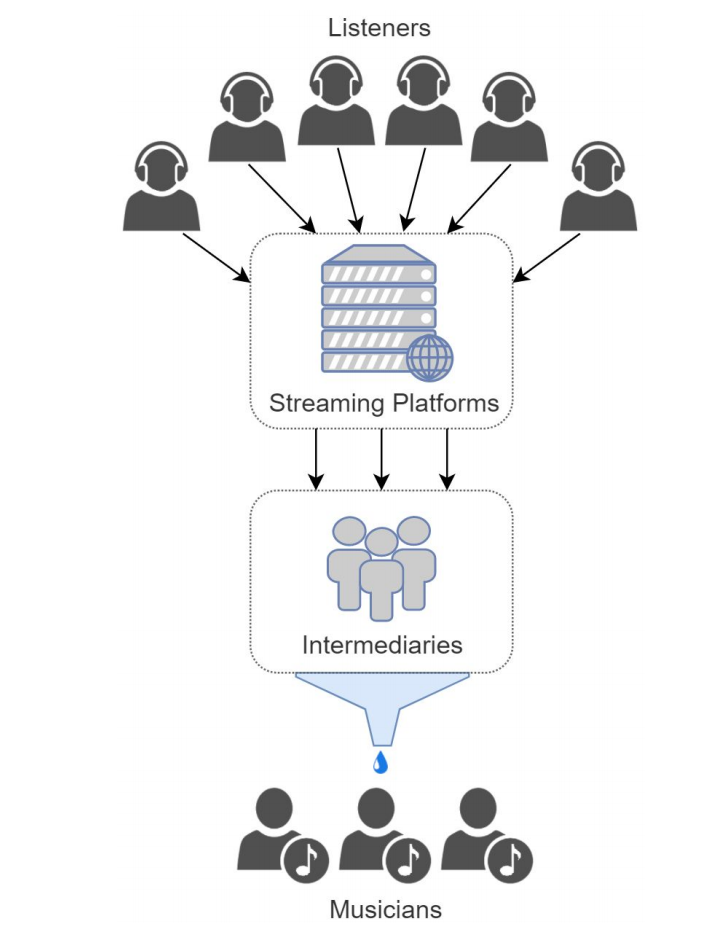
\includegraphics[width=0.4\textwidth]{introduction/problem-image.png}
	\caption{Artist compensation inconsistency}
\end{figure}

\section{Proposed solution: MusicDAO}
This thesis proposes an alternative technology from Big Tech streaming services. We design and implement a decentralized system which attempts to replace the full value chain in music streaming industry, from the subscription money to the artist, by removing all intermediaries and giving power back to the artists and listeners. Listeners can stream music without being dependent on a single provider and can give money directly to artists. Artists receive 100\% of this donation and subscription money.

In essence, the solution is a decentralized autonomous organization (DAO) which is formed by listeners and artists. A DAO is defined by \cite{buterin2014dao} as an ``entity that lives on the internet and exists autonomously, but also heavily relies on hiring individuals to perform certain tasks that the automaton itself cannot do'' (see \ref{fig:dao-quadrants}). In this thesis we present the design and implementation of our mobile android app MusicDAO: a music streaming service for the common good. Users of this app form a phone-to-phone zero-server network over which they publish music, download music and transfer money. This proof-of-principle of a DAO shows a fair and transparent music streaming service in which no external servers, third parties or intermediaries are necessary. Any person can join the network, publish music and get paid for it. 

MusicDAO supports the following functionalities:
\begin{itemize}
    \item Defining and publishing music content with metadata;
    \item Streaming music over BitTorrent;
    \item Caching and streaming optimization algorithms;
    \item Browsing playlists;
    \item Remote keyword search;
    \item Peer-to-peer donations to artists using Bitcoin.
\end{itemize}

\subsection{Experimentation and evaluation}
In a real-world experiment with Android phones, we tested the feasibility of such a phone-to-phone infrastructure-less system. We ran MusicDAO on at least X android devices, and registered the latency of retrieving music metadata, and transaction speeds of transferring money and audio files. 

\section{Towards a Robot Economy}
A full robot economy aims to have the following key characteristics: automation, transparency, fairness and democratic engagement. To accomplish these key characteristics in a software system, we envision the main building blocks to be as described in fig. \ref{tab:robot-economy-building-blocks}.

\begin{table}[]
\begin{tabular}{|l|l|}
\hline
\textbf{Component}                         & \textbf{Focus in MusicDAO} \\ \hline
Peer-to-peer leaderless infrastructure     & \checkmark                                      \\ \hline
Resilient communication                    & \checkmark                                      \\ \hline
Trustless content sharing and exploration  & \checkmark                                      \\ \hline
Trustless monetary system                  & \checkmark                                      \\ \hline
Democratic user engagement                      & $\times$                                      \\ \hline
AI for decision making (robot tasks)       & $\times$                                      \\ \hline
Continuous code evolution and distribution & $\times$                                       \\ \hline
\end{tabular}
\caption{The main components to achieve a robot economy in software}
\label{tab:robot-economy-building-blocks}
\end{table}

% Music artists have a hard time making a living. The oligarchical power of music streaming services and labels squeeze  the  production  size  of  the  music  industry
% Stolen from Resonate.is:
% The music industry is dysfunctional. Power has become consolidated in the hands of a small number of technology companies and dominant major labels.

% Section X describes the design of the system, section Y its implementation and Z its testing results.
% Most important: How can artists distribute and sell their work in a digital economy beholden to ruthlessly commercial and centralized interests?
% https://thebaffler.com/salvos/the-problem-with-muzak-pelly

% From Audius Whitepapter:
% We see a number of specific challenges faced by creatorsand listeners today:1.  There is little to no transparency around the originsof creator payouts (e.g.  number of plays, location,original gross payment before fees)2.  Incomplete  rights  ownership  data  often  preventscontent  creators  from  getting  paid;  instead,  earn-ings accumulate in digital service providers (DSPs)and rights societies3.  There are layers of middlemen and significant timedelay involved in payments to creators4.  Publishing rights are complicated and opaque, withno incentives for the industry to make rights datapublic and accurate5.  Remixes,  covers,  and  other  derivative  content  arelargely censored due to rights management issues6.  Licensing issues prevent DSPs and content from be-ing accessible worldwide
